\documentclass[a4paper,12pt]{article}

\usepackage[portuguese]{babel}
\usepackage{comment}
\usepackage[T1]{fontenc}
\usepackage[utf8]{inputenc}
\usepackage{hyperref}
\usepackage{graphicx}
\usepackage{float}
%\usepackage{multirow}
\usepackage[hypcap]{caption} % makes \ref point to top of figures and tables
\usepackage{amsmath}
%\usepackage[usenames,dvipsnames,svgnames,table]{xcolor}
%\usepackage{rotating}
\usepackage{subcaption}
\usepackage{listings}
\usepackage{color}
\usepackage[margin=0.95	in]{geometry} %margens da página
\usepackage{placeins}

\definecolor{keywordcolor}{rgb}{0,0.4,0.7}
\definecolor{commentcolor}{rgb}{0.4,0.4,0.4} 	
\definecolor{mygray}{rgb}{0.5,0.5,0.5} 	% line counter color
\definecolor{mymauve}{rgb}{0.55,0.28,0.62}	% string color
\definecolor{codebackground}{rgb}{0.95,0.95,0.95} 

\lstset{ %
  backgroundcolor=\color{codebackground},   % choose the background color; you must add \usepackage{color} or \usepackage{xcolor}
  basicstyle=\ttfamily \footnotesize,        % the size of the fonts that are used for the code
  breakatwhitespace=false,         % sets if automatic breaks should only happen at whitespace
  breaklines=true,                 % sets automatic line breaking
  captionpos=b,                    % sets the caption-position to bottom
  commentstyle=\color{commentcolor},    % comment style
  deletekeywords={...},            % if you want to delete keywords from the given language
  escapeinside={\%*}{*)},          % if you want to add LaTeX within your code
  extendedchars=true,              % lets you use non-ASCII characters; for 8-bits encodings only, does not work with UTF-8
  keepspaces=true,                 % keeps spaces in text, useful for keeping indentation of code (possibly needs columns=flexible)
  keywordstyle=\color{keywordcolor},       % keyword style
  numbers=left,                    % where to put the line-numbers; possible values are (none, left, right)
  numbersep=5pt,                   % how far the line-numbers are from the code
  numberstyle=\tiny\color{mygray}, % the style that is used for the line-numbers
  rulecolor=\color{black},         % if not set, the frame-color may be changed on line-breaks within not-black text (e.g. comments (green here))
  showspaces=false,                % show spaces everywhere adding particular underscores; it overrides 'showstringspaces'
  showstringspaces=false,          % underline spaces within strings only
  showtabs=false,                  % show tabs within strings adding particular underscores
  stepnumber=1,                    % the step between two line-numbers. If it's 1, each line will be numbered
  stringstyle=\color{mymauve},     % string literal style
  tabsize=2                       % sets default tabsize to 2 spaces
}

\renewcommand{\lstlistingname}{Código}	% Listing x -> Código x
\def\lstlistingautorefname{Código}



\begin{document}

\pagenumbering{gobble}
\begin{titlepage}

	\begin{center}

		
\includegraphics[width=6cm]{./title}\\[3cm]

		\textsc{\LARGE Electrónica de Computadores}\\[1.5cm]

		\textsc{\Large Projecto 2}\\[1.5cm]


		{ \huge \bfseries Processamento de Imagem no Processador Softcore MicroBlaze\\[2.5cm] }


		\noindent
		\begin{center} \large
			Gonçalo Ribeiro, 73294\\[5mm]

			Ricardo Amendoeira, 73373\\[5mm]

			Rafael Gonçalves, 73786\\[2.5cm]

			\textit{Docente: Prof. Francisco Alegria}

		\end{center}

		\vfill

		{\large \today}

	\end{center}

\end{titlepage}

\tableofcontents
\pagebreak

\pagenumbering{arabic}
\section{Introdução}
Este projecto tem como principal objectivo fazer processamento de imagem em tempo real recorrendo a uma placa Digilent S3 e a uma câmara com interface VGA. A placa Digilent S3 é uma placa de prototipagem com FPGA que nos permite implementar um processador MicroBlaze. O MicroBlaze comunica com a câmara para fazer o processamento da imagem capturada, que é mostrada num monitor através da saída VGA do dispositivo.

A realização do projecto permitirá a aprendizagem de como implementar um \textit{general purpose processor} como o MicroBlaze numa FPGA, como programar (pelo software providenciado pela Xilinx\textregistered) e utilizar periféricos com esse processador (neste caso a câmara e a interface VGA). Aprendemos também como fazer algumas operações simples de processamento de imagem, Histograma e Embossing.


\section{Material Utilizado}
\subsection*{Hardware}
\begin{itemize}
\item câmara de 1.3 Mpx ($1280\times1024\times24$) e \textit{breakout board}
\item computador com Xilinx EDK
\item placa Digilent S3 com Xilinx FPGA XC3S1000-4
\item monitor com entrada VGA
\end{itemize}

Uma FPGA (\textit{Field Programmable Gate Array}) é um circuito integrado desenhado para ser configurado pelo utilizador depois do fabrico de forma a implementar circuitos digitais. Estes circuitos são normalmente desenhados por via de uma linguagem de descrição de \textit{Hardware} como VHDL ou Verilog. O utilizador pode depois usar o \textit{software} fornecido pelo fabricante para traduzir o circuito e configurar a FPGA utilizada. Estes dispositivos contêm muitos blocos lógicos, como LUT's, portas lógicas simples, somadores e multiplicadores, que podem ser activados e ligados entre si de várias formas para implementar o circuito desejado. Podem também ter funções analógicas como DAC's e ADC's. Estas capacidades tornam as FPGA's num dispositivo extremamente útil para a prototipagem de circuitos digitais ou implementações de baixo custo em produtos fabricados em pequenas quantidades.   

A placa usada neste projecto, a Digilent S3,  inclui uma FPGA Xilinx FPGA XC3S1000-4 e conta com 8 LEDs que são usados numa fase inicial do trabalho (Secção~\ref{subsec:LEDs}). Conta também com 3 conjuntos de 40 pinos, um dos quais é usado para ligar a placa da câmara à da FPGA.

\subsection*{Software}
O software utilizado neste projecto foi o Xilinx Platform Studio (XPS) e o Xilinx Software Development Kit (SDK), ambos incluídos no Xilinx Embedded Development Kit (EDK). No XPS são feitas as ligações e algumas configurações da FPGA e no SDK é desenvolvido o software para o MicroBlaze.

\section{Layout e especificações do Projecto}

A FPGA utilizada é uma Xilinx XC3S1000-4, isto é, uma FPGA da família Spartan-3, com 1000K (ou seja, 1M) portas de sistema, com \textit{Speed Grade} de -4, que corresponde a \textit{Standard Performance}. O relógio de sistema funciona a 326 MHz, existindo no dispositivo 4 \textit{Digital Clock Managers}, cada um equipado com um \textit{Delay Locked Loop}.

\begin{figure}[h]
	\centering	
	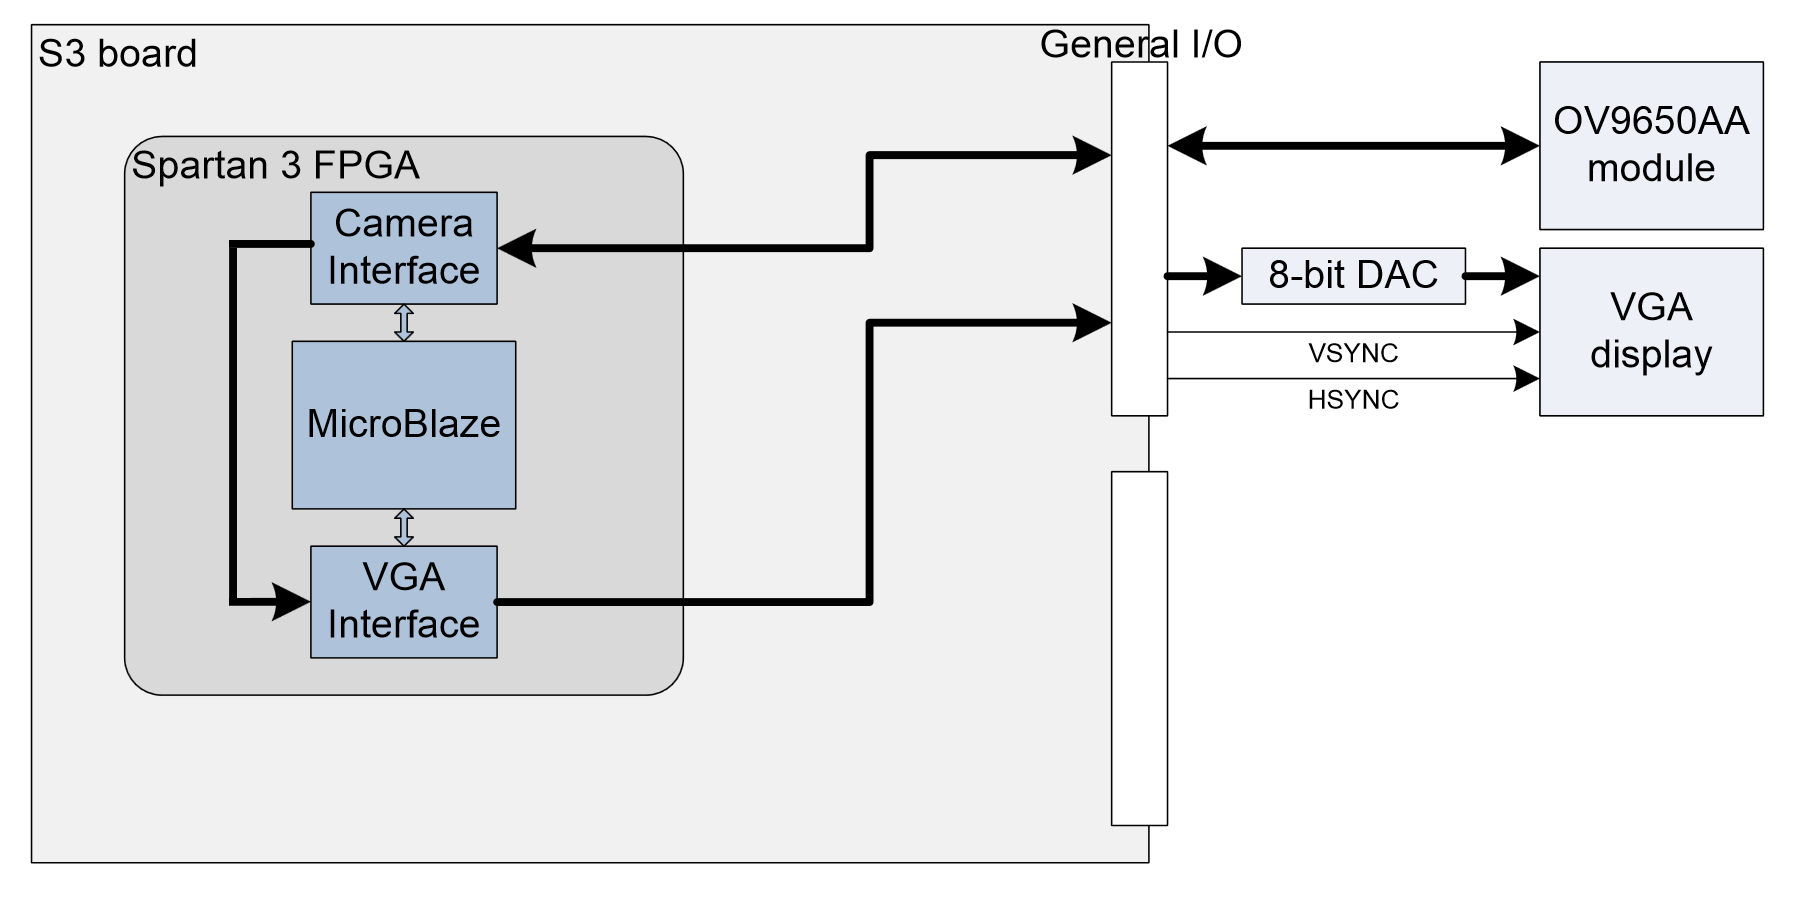
\includegraphics[scale = 0.3]{imagens/esquema_projecto.png}
	\caption{Esquema geral do sistema}
	\label{fig:esquemaGeral}
\end{figure}
\FloatBarrier

A câmara é configurada para trabalhar com uma resolução de $128\times64$ píxeis, e o monitor para mostrar a imagem directamente da câmara, bem como o resultado do processamento que sai do MicroBlaze implementado na FPGA. O monitor é ligado através de uma ligação VGA e sendo esta uma ligação analógica é necessária a utilização de um \textit{Digital to Analog Converter} (DAC) entre os pinos de \textit{I/O} da placa e a ligação ao monitor. O DAC usado no projecto é uma escada de resistências  com 8 bits, esquema na figura abaixo: 

\begin{figure}[h]
	\centering	
	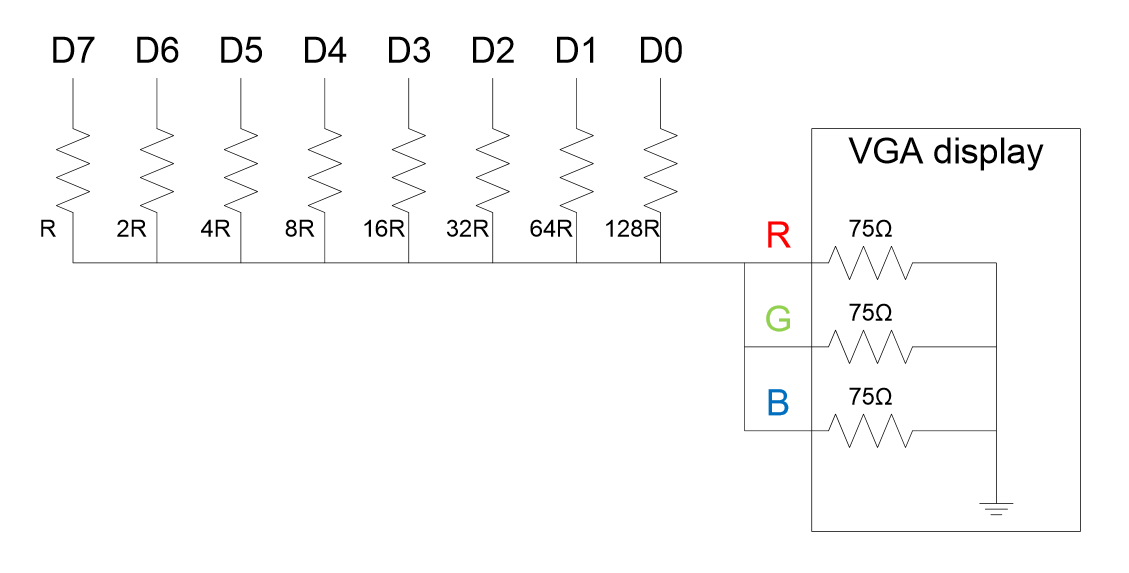
\includegraphics[ scale=0.4]{imagens/esquema_dac.png}
	\caption{DAC usado no projecto}
	\label{fig:esquemaDAC}
\end{figure}
\FloatBarrier

O microprocessador MicroBlaze trata-se de uma arquitectura de 32 bits, desenhada para implementação em FPGAs proprietárias da Xilinx. O ambiente de desenvolvimento disponibilizado permite configurar as ligações do sistema e dos barramentos de dados, bem como executar binários compilados no próprio ambiente.



\section{Implementação do Projecto}
\subsection{Introdução à FPGA}
\label{subsec:LEDs}
% LEDs a piscar

Esta parte introdutória do projecto pretende uma familiarização com os ambientes de desenvolvimento e a configuração inicial da FPGA de forma a se ter uma melhor preparação para as fases subsequentes do trabalho. Para isso é criado um projecto que visa a implementação de software no processador \textit{softcore} MicroBlaze. O software a implementar permite controlar os LEDs da placa.

Começa-se por criar um novo projecto usando o Xilinx Platform Studio. De seguida, há que definir para que placa e FPGA estamos a desenvolver e ainda qual a \textit{package} e o \textit{speedgrade}. O tipo de interligações escolhido para fazer a interface entre o processador e os dispositivos é PLB (\textit{processor local bus}). Define-se também que o tipo de processador a usar é MicroBlaze a funcionar a uma frequência de 50 MHz e com 32 KB de memória e sem cache.

Até agora o sistema não tem qualquer periférico. O passo seguinte é adicionar um periférico que permita fazer chegar o sinal de controlo do MicroBlaze aos LEDs da placa. Para controlar o LEDs é usado um periférico que já vem definido no catálogo de propriedade intelectual do XPS (IP Catalog): o \textit{XPS General Purpose IO}. A largura deste módulo deverá ser de 8 bits visto que é esse o número de LEDs que existe na placa.

Uma vez criado o periférico é preciso ligá-lo à PLB para que possa comunicar com o MicroBlaze e tornar externas as portas deste dispositivo. De seguida há que reservar uma região da memória do MicroBlaze para comunicação com o novo periférico. Essa região pode ser escolhida automaticamente pelo XPS.

Antes de gerar o \textit{bitstream} falta ainda alterar o ficheiro \texttt{.ucf} para impor as \textit{contraints} adequadas ao projecto, como a frequência de operação e o mapeamento para as portas externas. Neste cado o ficheiro \texttt{.ucf} adequado é fornecido pelos docentes. O \textit{bitstream} pode agora ser gerado (note-se que este processo é demorado, cerca de 10 minutos) e após isso pode exportar-se as configurações de hardware para o SDK. A partir deste ponto o desenvolvimento é feito no SDK.

Está-se agora apto a implementar o software que se queira correr no MicroBlaze. No SDK cria-se um novo \textit{Board Support Package} e um projecto em C a que se adiciona um ficheiro de código \texttt{main\_leds.c}. Após a escrita do código há que gerar o \textit{Linker Script}, que permitirá gerar o executável.

Está tudo preparado para programar a FPGA e correr o executável. Neste caso se tudo for feito correctamente os LEDs da placa deverão acender e apagar sequencialmente como que fazendo um \textit{rotate} de um bit.

%\lstinputlisting[language=C, label=code:main_leds, caption=\texttt{main\_leds.c} após alteração]{codigo/main_leds.c}

É pedido que o código do ficheiro \texttt{main\_leds.c} seja alterado de forma a que o \textit{rotate} seja feito no sentido contrário ao original, o que é uma alteração simples, bastando mudar o sentido do shift e alterar a condição de reset.  %O código após essa alteração é o \autoref{code:main_leds} e funcionou como previsto.

Este código começa por inicializar a \textit{driver} do periférico GPIO e definir todos os seus sinais como outputs. De seguida, a execução fica presa num ciclo que cada vez que é executado faz um \textit{rotate} para a direita e depois o MicroBlaze escreve o novo valor para o periférico, que polariza os LEDs apropriadamente. É usado um \textit{delay} entre iterações do ciclo para que os LEDs possam ser vistos a mudar em vez de aparentarem estar todos acesos (com menor intensidade). Este \textit{delay} é feito com um ciclo que faz uma contagem de \texttt{0} ao valor de \texttt{LED\_DELAY}. Como este ciclo está vazio é importante que o código seja compilado sem optimizações porque caso contrário este ciclo pode ser suprimido e os LEDs não terão o comportamento previsto.

\subsection{Interface com a Câmara e saída VGA}
% preparação da câmara para usar nas fases seguintes

O trabalho desta secção é construído sobre o projecto criado na Secção~\ref{subsec:LEDs}. No XPS, começa-se por adicionar nova IP fornecedida em conjunto com o enunciado. Os periféricos adicionados à \textit{bus} são \texttt{VGA\_interface} e \texttt{camera\_interface}, que se referem respectivamente à câmara e ao monitor VGA. São depois adicionadas duas \textit{buses} FSL (\textit{fast simplex link}). O motivo pelo qual se usam \textit{buses} FSL é a aplicação a desenvolver ser uma \textit{time-critical application}. Segundo as app notes do Xilinx, nestes casos deve ser usado a \textit{bus} FSL em vez da OPB (\textit{on-chip peripheral bus}) para integrar a IP no MicroBlaze. Fazendo isto é depois possível utilizar funções em C para usar IP adicionada pelo utilizador (neste caso \texttt{VGA\_interface} e \texttt{camera\_interface}).

O MicroBlaze é configurado para usar um multiplicador de 32 bits, divisão inteira e uma \textit{stream} FSL. De seguida, fazem-se as interligações necessárias entre o MicroBlaze, a interface VGA e a câmara. São ainda actualizadas as \textit{constraints} do ficheiro \texttt{.ucf} do projecto. Gera-se a \textit{bitstream}, que é exportada para o SDK.

Da mesma forma que na Secção~\ref{subsec:LEDs} foi adicionado o ficheiro \texttt{mail\_leds.c}, no SDK adiciona-se agora o ficheiro \texttt{negative.c}. Liga-se a Digilent S3 à placa da câmara, programa-se a FPGA e corre-se o software. No monitor vê-se a imagem da câmara e por baixo a mesma imagem mas com escala de cinzentos invertida.

O código do \texttt{negative.c} não é aqui incluído porque não foi alterado. No entanto esse código serve de base para o trabalho realizado nas Secções~\ref{subsec:histograma}~e~\ref{subsec:relevo}.

\subsection{Processamento de Imagem por Software}
\subsubsection{Histograma}
\label{subsec:histograma}

Nesta parte do trabalho pretendemos implementar uma aplicação que faça um histograma dos níveis de cinzento da imagem capturada. A imagem capturada tem como dimensões $128\times64\times256$, ou seja 128 bits de largura, 64 de altura e 256 níveis de cinzento.

O histograma deverá ser uma representação gráfica do número de vezes que cada nível de cinzento aparece numa imagem capturada. Para fazer esta contagem a imagem tem que ser varrida e um vector de contagens é inializado a zero e depois incrementado de acordo com o varrimento que é feito.

Como já referido a imagem que é capturada tem 256 níveis de cinzento. No monitor a área que temos para representar o histograma é de $128\times64$ px. Escolhe-se então o eixo horizontal para fazer a representação de cada valor de cinzento---visto que permite representar mais valores---e o vertical para o número de contagens. No entanto a resolução do eixo horizontal não chega para representar todos os tons. Consequentemente é preciso colapsar dois tons de cinzento para uma mesma coluna do monitor. Convenciona-se então que cada coluna do monitor representa o valor de dois tons de cinzento consecutivos, i.e.\ no índice \texttt{0} do vector \texttt{histogram} do \autoref{code:histograma} encontram-se as contagens dos níveis de cinzento \texttt{0} e \texttt{1}; no índice \texttt{1} as contagens dos tons \texttt{2} e \texttt{3}; e assim por diante.

\clearpage
\lstinputlisting[language=C,label=code:histograma, basicstyle=\footnotesize, caption={histogram (pseudo-código)}]{codigo/histogram.c}


O número máximo de contagens que pode existir para cada tom de cinzento é $128\times64 = 2^{13}$, pelo que cada valor do vector \texttt{histogram} tem que ter pelo menos 13 bits, o que numa arquitectura de 32 bits corresponderia ao tipo \texttt{short}. O facto de no monitor termos apenas 64 linhas para representar o número de contagens leva a que seja preciso multiplicar por um factor de escala cada contagem. Isso poderia ser feito com um factor de escala constante com a desvantagem de que em algumas situações pode ser difícil visualizar algumas barras dependendo da calibração escolhida para esse factor de escala. Outra abordagem é o factor de escala ser escolhido dinamicamente, ou seja ser escolhido de forma a que a contagem máxima em cada instante preencha os 64 px de altura. Com esta abordagem temos a desvantagem de que ao ser varrida a imagem temos que calcular qual os dois tons consecutivos com o máximo de ocorrências; e não é possível comparar quantitativamente as várias imagens recolhidas por não terem a mesma escala. Escolheu-se um factor de escala dinâmica por permitir uma representação mais versátil.

A implementação por software é relativamente simples (ver \autoref{code:histograma}). A imagem começa por ser recebida pela \textit{bus} FSL e guardada no vector \texttt{image}. De seguida é feito um varrimento linear de \texttt{image} e são obtidas as contagens para tons de cinza consecutivos. De seguida é feita a normalização das contagens, o que envolve descobrir qual o grupo de tons com o máximo de contagens e escalar todas as contagens.

\clearpage
Resta preencher o vector \texttt{outimage} com a representação do histograma que será vista no monitor. Para isso basta varrer \texttt{outimage} escrevendo em cada índice \texttt{0} (preto) nas regiões cujo número da linha esteja abaixo ou seja igual ao número de contagens; e \texttt{255} (branco) nos pixeis das regiões acima do número de contagens. Isto resulta num histograma preto sobre fundo branco. \texttt{outimage} está assim pronta a ser enviada via FSL para a interface VGA do monitor.

\begin{figure}[h]
	\centering
	\begin{subfigure}[b]{0.40\textwidth}
		\centering
		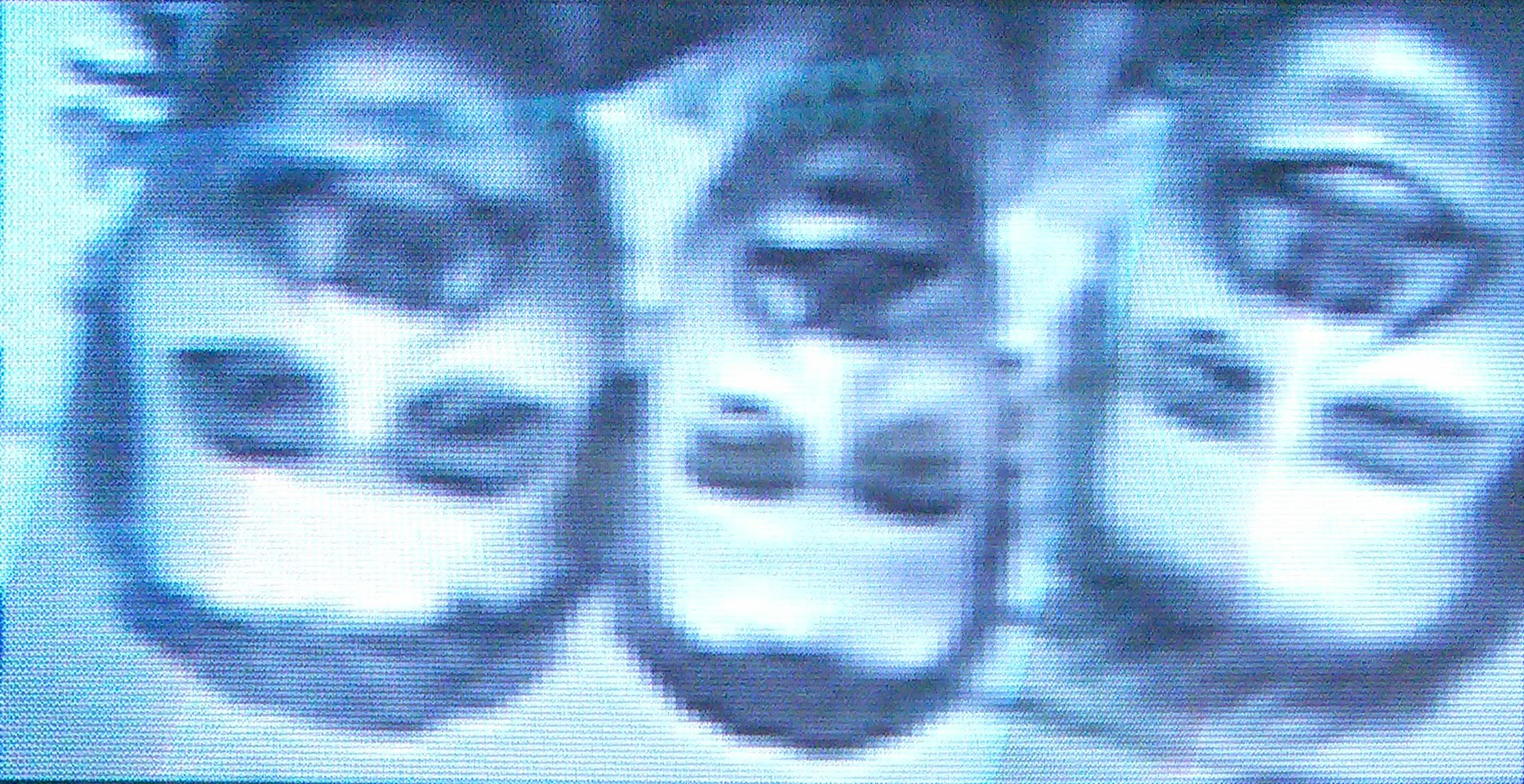
\includegraphics[width=\linewidth]{imagens/hist_capturada.png}
		\caption{}
		%\label{fig:}
	\end{subfigure}
	\begin{subfigure}[b]{0.40\textwidth}
		\centering
		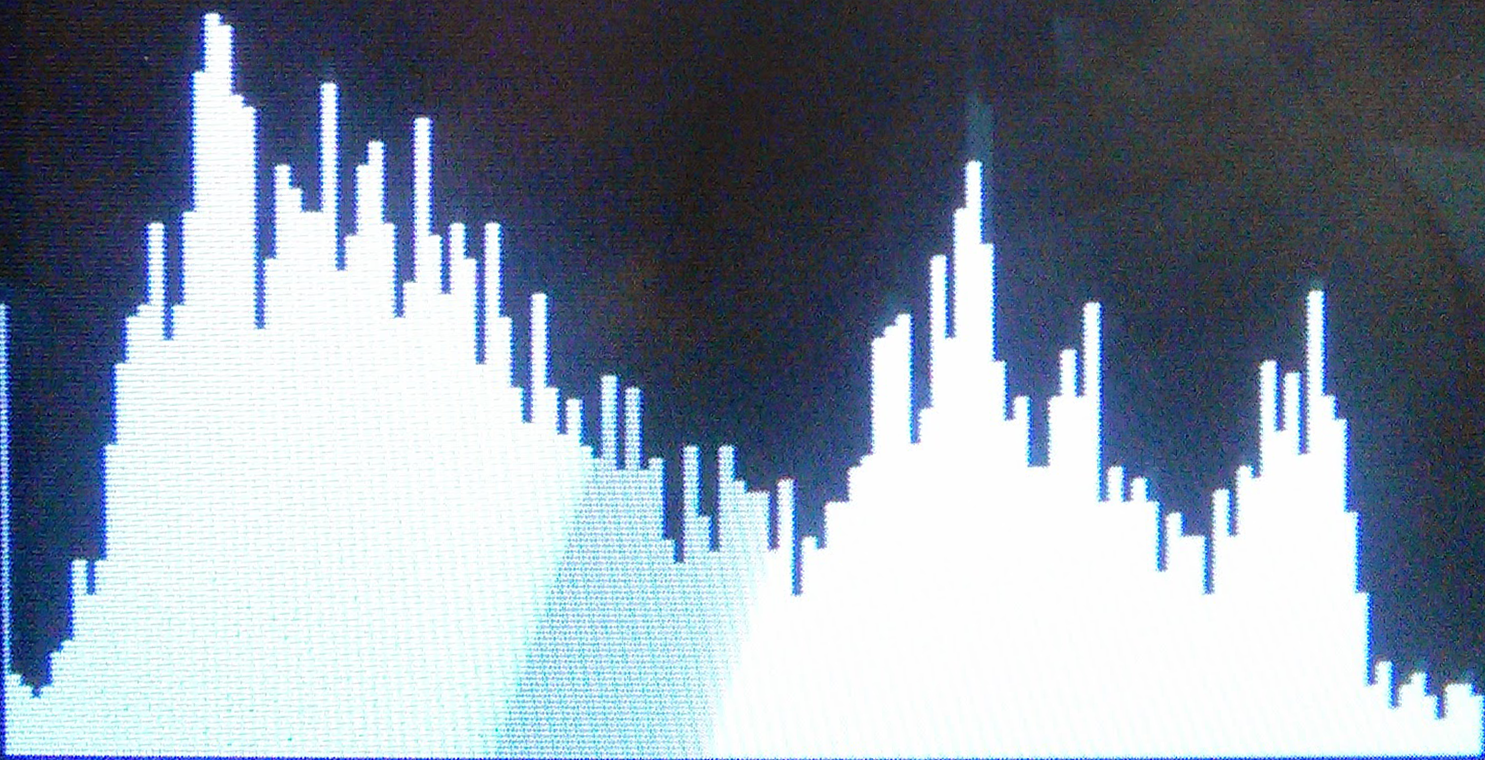
\includegraphics[width=\linewidth]{imagens/hist_resultado.png}
		\caption{}
		%\label{fig:}
	\end{subfigure}
	\caption{(a) imagem capturada e (b) respectivo histograma (as riscas diagonais não fazem parte da imagem, são um artefacto do método de captura)}
	\label{fig:histograma}
\end{figure}


\subsubsection{Relevo (\textit{embossing})}
\label{subsec:relevo}

O algoritmo especificado no enunciado é o seguinte:

\[
D' = K \ast I
\]

\[
D = D' - \widetilde{K} \ast I
\]

Onde $I$ é uma matriz $3 \times 3$ que contém a informação relativa a um pixel e aos 8 píxeis adjacentes.

\[ K =
\begin{bmatrix}
-2 & -2 & 0\\
-2 & 6 & 0\\
0 & 0 & 0
\end{bmatrix}
\]

\[\widetilde{K} = 
\begin{bmatrix}
0&0&0\\
0&-6&2\\
0&2&2
\end{bmatrix}
\]

De maneira a não alocar a memória necessária a um buffer intermédio (uma vez que isso excedia as capacidades do dispositivo), compactámos o algoritmo da seguinte maneira:

\[
D = K \ast I - \widetilde{K} \ast I
\]

Como $K_{i,j} = \widetilde{K}_{(2-j),(2-i)}$, fizemos a simplificação adicional de não construir a matriz $\widetilde{K}$. Como as duas matrizes possuem uma linha e uma coluna de zeros, o espaço alocado para a matriz foi $2\times2$ em vez de $3\times3$. O algoritmo foi, consequentemente, adaptado.

\clearpage
\lstinputlisting[language=C,label=code:embossing, basicstyle=\footnotesize,  caption={embossing (pseudo-código)}]{codigo/embossing.c}

Uma vez feitas as operações sobre os dados, o resultado é normalizado, de maneira a que o valor mais claro corresponda a um píxel branco, e o mais escuro a um píxel preto.

Cada píxel exige dados relativos aos 8 píxeis adjacentes, pelo que há duas linhas e colunas (nas margens) que não recebem informação suficiente e consequentemente não têm significado.

\begin{figure}[h]
	\centering
	\begin{subfigure}[b]{0.40\textwidth}
		\centering
		\includegraphics[width=\linewidth]{imagens/emb_capturada.png}
		\caption{}
		%\label{fig:}
	\end{subfigure}
	\begin{subfigure}[b]{0.40\textwidth}
		\centering
		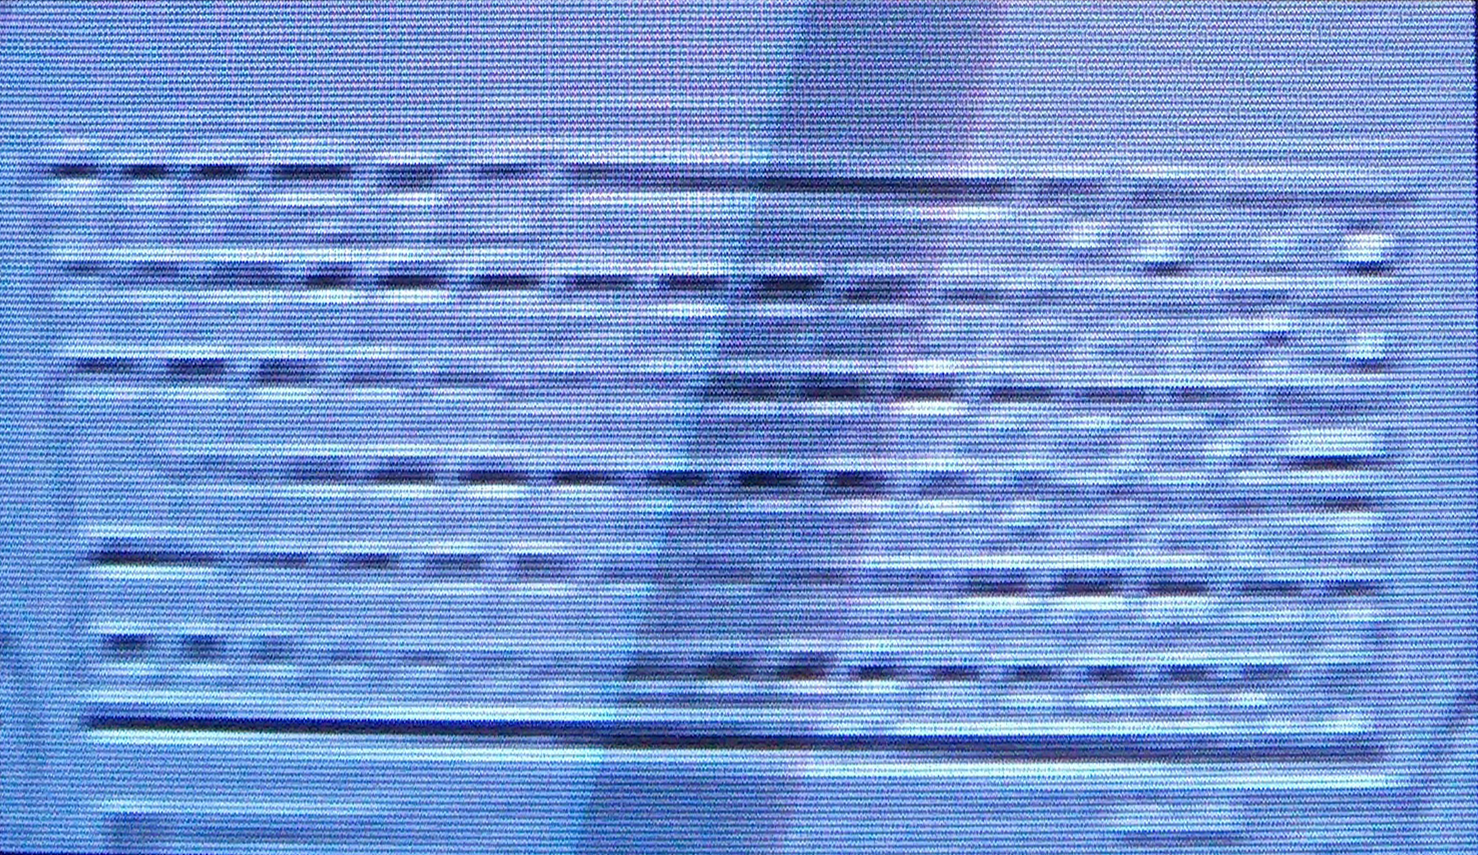
\includegraphics[width=\linewidth]{imagens/emb_resultado.png}
		\caption{}
		%\label{fig:}
	\end{subfigure}
	\caption{(a) imagem capturada e (b) respectivo relevo (as riscas diagonais não fazem parte da imagem, são um artefacto do método de captura)}
	\label{fig:relevo}
\end{figure}
\FloatBarrier

\subsection{Processamento de Imagem por Hardware}
Na parte final do projecto alterou-se um ficheiro de VHDL para usar uma solução por hardware da computação do histograma nas configurações do nosso sistema. O ficheiro fornecido fazia o cálculo para 256 tons de cinzento diferentes, o que teve de ser alterado para caber nas 128 linhas que temos disponíveis no sistema de \textit{display}. A versão original do ficheiro fazia a contagem por via de uma BRAM com 256 endereços, cada um com o número de ocorrências do tom respectivo. Quando um tom era encontrado, a posição de memória respectiva era incrementada. Do lado do \textit{MicroBlaze} eram lidas as 256 posições e feito a apresentação da informação no \textit{display}. 

Como na implementação por software, combinámos os tons dois a dois, pelo que cada linha \textit{i} do histograma representa o tons de cinzento \textit{2i} e \textit{2i+1}. Os incrementos passaram assim a ser feitos em apenas 128 endereços da BRAM e o \textit{MicroBlaze} passou a ler apenas esses 128 endereços. Esta solução reduz a metade o número de leituras feitas pelo \textit{MicroBlaze}, melhorando a performance.

%Código do VHDL alterado: 

%NÃO ESQUECER 

\subsubsection{Implementação}

O ficheiro VHDL incluído no arquivo de laboratório fornecido pela docência foi alterado, uma vez que contava as ocorrências dos 256 tons de cinzento possíveis, em vez de agrupar os tons por pares, de maneira a perfazer um histograma de 128 colunas.

Assim, foram alteradas as linhas 315, 330 e 368.

Nas linhas 315 e 368, foram alterados os critérios dos ciclos de maneira a terminarem ao atingir 127, em vez de 255, e na linha 330 foi feito o dito agrupamento dos valores por pares.

\lstinputlisting[language=VHDL,label=code:hardhist, basicstyle=\footnotesize,  caption={Contexto da linga 315},firstline=315, lastline=321, firstnumber=315]{../camera_interface.vhd}

\lstinputlisting[language=VHDL,label=code:hardhist, basicstyle=\footnotesize,  caption={Contexto da linha 330},firstline=329, lastline=343, firstnumber=329]{../camera_interface.vhd}

\lstinputlisting[language=VHDL,label=code:hardhist, basicstyle=\footnotesize,  caption={Contexto da linha 368},firstline=368, lastline=374, firstnumber=368]{../camera_interface.vhd}

\subsection{Análise de Resultados}
Nenhuma das implementações conseguiu fazer o processamento em tempo real, várias frames eram descartadas porque o buffer era reescrito antes de ser feito o respectivo processamento. Ainda assim as implementações tinham uma fluidez aceitável, sendo possível seguir movimentos em frente à câmara.

A implementação por hardware do histograma era notoriamente mais fluída que por software. Para comparar a performance de ambas as implementações o código foi preparado para que a cada nova frame processada se acendesse o próximo LED, fazendo um \textit{rotate} como no exemplo da secção 4.1. Foram feitos dois vídeos de cerca de 10 segundos, um para cada implementação, a filmar os LED's da placa. Posteriormente foi feita uma média de quantas frames por segundo cada implementação era capaz. Chegou-se à conclusão de que a implementação por hardware era cerca de 30\% mais rápida. O valor calculado é no entanto menor que na realidade, uma vez que ambas as implementações têm o overhead acrescido de controlar os LED's e enviar as frames resultantes para a saída VGA, que é igual em ambas e diminui o impacto da melhoria.

\section{Conclusão e Observações}
Embora o projecto não utilidade prática na forma em que foi implementado (demasiados componentes de grande dimensão necessários para poder usar, com lenta iniciação) o valor lúdico é importante. Não seria complexo, no entanto, alterar o sistema usado para um de dimensões muito inferiores e de mais prática utilização. 

A volatilidade da memória da placa obriga a utilização de um computador com o software de programação instalado cada vez que se quer iniciar o sistema. Se for utilizado um tipo de memória não volátil, é possível retirar o computador do sistema. O monitor pode ser trocado por um LCD moderno de muito menores dimensões sem qualquer tipo de redesenho do sistema, desde que tenha uma interface VGA. Finalmente, todo o sistema pode tornar-se portátil com o uso de uma bateria, uma vez que os componentes necessários têm baixo consumo, sendo ainda mais prático se se recorrer a uma placa de prototipagem de menores dimensões. No caso da solução VHDL é ainda possível, embora caro em pequenas quantidades, implementar o hardware descrito pelo código. 

Estas alterações são relativamente simples e aumentariam muito a utilidade prática do projecto, se a intenção fosse a de criar um produto. 
Foi notada a baixa performance da implementação por software, que está limitada pela arquitectura do MicroBlaze e também pela performance da placa onde o MicroBlaze foi implementado. A versão VHDL permite ganhos significativos de performence ao custo de maior complexidade de implementação.   

No caso deste projecto a implementação por hardware seria claramente a mais adequada para um produto. O processamento feito é relativamente simples, o que diminui a vantagem do uso de um\textit{general purpose processor}, que é menos eficiente e tem uma performance inferior. É também relativamente fácil de paralelizar ambos os tipos de processamento, o que é ideal para implementações hardware. Na nossa opinião, a utilização de um \textit{general purpose processor} para a implementação final do sistema só seria justificada se a produção fosse de escala extremamente reduzida.

Voltando ao objectivo lúdico do projecto, permitiu comparar as vantagens e desvantagens de implementações por hardware e software, assim como aprender vários dos componentes e programas utilizados e entender como são feitos os tipos de processamento de imagem implementados. 


\bibliographystyle{plain}
\nocite{labsECom}
\bibliography{xilinx,labsECom}	% no spaces between commas!

\end{document}
